\documentclass[../TDE6_rsf.tex]{subfiles}%

\begin{document}
\section[s]"3"{Déphasage, pulsation et impédance}
\QR{%
	\begin{minipage}[t]{0.55\linewidth}
		On considère le circuit ci-contre en RSF. Déterminer l'expression de la
		pulsation $\w$ de la tension sinusoïdale $e(t) = E\cos(\wt)$ pour que le
		courant $i(t)$ soit en phase avec $e(t)$. Déterminer alors une condition sur
		$R_2$, $C$ et $L$ pour que cela soit réalisable.
		\bigbreak
		\textit{Indication}~: utiliser l'impédance équivalente constituée de $C$,
		$L$ et $R_2$.
	\end{minipage}
	\hfill
	\begin{minipage}[t]{0.40\linewidth}
		\vspace{0pt}
		\begin{center}
			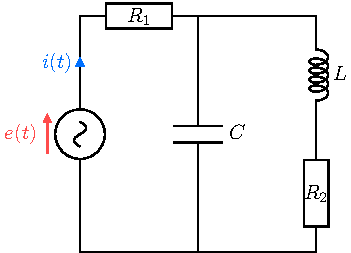
\includegraphics[width=\linewidth]{dephasage_rc_parr_lr_plain}
		\end{center}
	\end{minipage}
}{%
	Pour exprimer simplement $i$, il nous faut une seule maille avec une seule
	impédance équivalente $\Zu\ind{eq}$~: de cette manière, la loi des mailles nous
	donnera $\Eu = \Zu\ind{eq}\xul{I}$ et on pourra facilement déterminer le
	déphasage entre $i$ et $e$.
	\vspace{-15pt}
	\begin{center}
		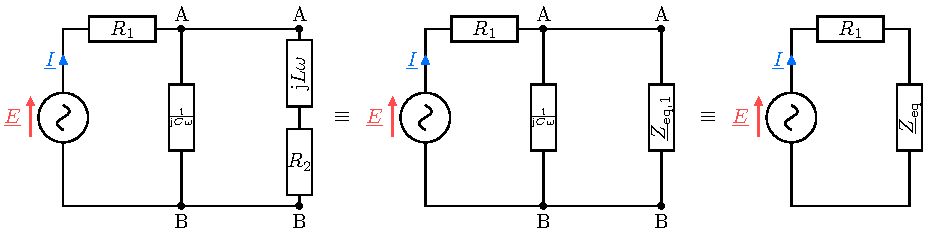
\includegraphics[width=\linewidth]{dephasage_rc_parr_lr_equiv}
	\end{center}
	On calcule l'impédance équivalente de l'association en série de $R_2$ et $L$~:
	\[\Zu\ind{eq,1} = R_2 + \jj L\w\]
	Cette association est en parallèle avec $C$~:
	\begin{gather*}
		\Zu\ind{eq, 2}
		= \frac{\Zu_C\times\Zu\ind{eq, 1}}{\Zu_C + \Zu\ind{eq,1}}
		= \frac{\dfrac{1}{\jj C\w}(R_2 + \jj L\w)}{\dfrac{1}{\jj C\w} + R_2 +
			\jj L\w}\\
		\Lra
		\Zu\ind{eq,2} = \frac{R_2 + \jj L\w}{1+\jj R_2C\w - LC\w^2}
	\end{gather*}
	On a donc comme prévu avec la loi des mailles~:
	\[\boxed{\xul{I} = \frac{\Eu}{R_1 + \Zu\ind{eq,2}}}\]
	L'intensité est en phase avec la tension si $\arg{R_1 + \Zu\ind{eq,2}} = 0$.
	Pour étudier cet angle, on va l'écrire sous la forme [partie réelle + $\jj $
			partie imaginaire]~; en effet, on aura alors
	\[
		\arg*{R_1 + \Zu\ind{eq,2}} = 0
		\Lra
		\tan(\arg*{R_1 + \Zu\ind{eq,2}}) = 0
		\Lra
		\boxed{\Im(R_1 + \Zu\ind{eq,2}) = 0}
	\]
	si la partie réelle est positive.
	\begin{align*}
		\beforetext{Ainsi~:}
		R_1 + \Zu\ind{eq,2} & =
		R_1 + \frac{R_2 + \jlw}{1 - LC\w^2 + \jj R_2C\w} \times
		\ora{\frac{1 - LC\w^2 \boxed{-}\jj R_2C\w}{1 - LC\w^2 \boxed{-}\jj R_2C\w}}
		\\
		                    & =
		R_1 +
		\frac{%
			(R_2+\jlw)\cdot (1 - LC\w^2 - \jj R_2C\w)
		}{%
			(1-LC\w^2)^2 + (R_2C\w)
		}
		\\&=
		R_1 + \frac{%
		R_2 (1-LC\w^2)-\jj R_2{}^2C\w + \jlw (1-LC\w^2) + LR_2C\w^2
		}{%
		(1-LC\w^2)^2 + (R_2C\w)
		}
		\\&=
		R_1 +
		\frac{R_2 (1-\cancel{LC\w^2}) + \cancel{LR_2C\w^2}}{(1-LC\w^2)^2 + (R_2C\w)} +
		\jj \frac{L\w (1-LC\w^2) -R_2{}^2C\w}{(1-LC\w^2)^2 + (R_2C\w)}
		\\&=
		\underbracket[1pt]{R_1 + \frac{R_2}{(1-LC\w^2)^2 + (R_2C\w)}}_{\Re > 0} +
		\jj \frac{L\w (1-LC\w^2) -R_2{}^2C\w}{(1-LC\w^2)^2 + (R_2C\w)}
	\end{align*}
	\begin{isd}
		On cherche donc
		\begin{align*}
			\Im(R_1 + \Zu\ind{eq,2}) & = 0
			\\\Lra
			L \cancel{\w} (1-LC\w^2) & = R_2{}^2C \cancel{\w}
			\\\Lra
			L - L^2 C\w^2            & = R_2{}^2C
			\\\Lra
			L^2C\w^2                 & = L - R_2{}^2C
			\\\Lra
			\w^2                     & = \frac{1}{LC} - \frac{R_2{}^2}{L^2}
			\\\Lra
			\Aboxed{%
			\w                       & = \sqrt{\frac{1}{LC} - \frac{R_2{}^2}{L^2}}
			}
		\end{align*}
		\tcblower
		Ceci est possible si le terme sous la racine est positif, soit
		\begin{align*}
			\frac{1}{LC}       & > \frac{R_2{}^2}{L_2}
			\\\Lra
			\cancel{L}C        & < \frac{L^{\cancel{2}}}{R_2{}^2}
			\\\Lra
			\Aboxed{%
			\frac{R_2{}^2C}{L} & < 1
			}
		\end{align*}
	\end{isd}
	\vspace{-15pt}
}
\end{document}
